\section{【背景】Intel
80386加电后启动过程}\label{ux80ccux666fintel-80386ux52a0ux7535ux540eux542fux52a8ux8fc7ux7a0b}

\textbf{【要点(非OSP):80836物理内存地址空间】}

\textbf{【要点(非OSP):80836加电后的第一条指令位】}

大家一般都知道bootloader负责启动操作系统,但bootloader自身是被谁加载并启动的呢?为了追根溯源,我们需要了解当计算机加电启动后,到底发生了什么事情。

对于绝大多数计算机系统而言,操作系统和应用软件是存放在磁盘(硬盘/软盘)、光盘、EPROM、ROM、Flash等可在掉电后继续保存数据的存储介质上。当计算机加电后,一般不直接执行操作系统,而是一开始会到一个特定的地址开始执行指令,这个特定的地址存放了系统初始化软件,通过执行系统初始化软件(可固化在ROM或Flash中,也称firmware,固件)完成基本I/O初始化和引导加载操作系统的功能。简单地说,系统初始化软件就是在操作系统内核运行之前运行的一段小软件。通过这段小软件的基本I/O初始化部分,我们可以初始化硬件设备、建立系统的内存空间映射图,从而将系统的软硬件环境带到一个合适的状态,以便为最终调用操作系统内核准备好正确的环境。最终系统初始化软件的引导加载部分把操作系统内核映像加载到RAM中,并将系统控制权传递给它。

对于基于Intel 80386的计算机而言,其中的系统初始化软件由BIOS (Basic Input
Output
System,即基本输入/输出系统,其本质是一个固化在主板Flash/CMOS上的软件)和位于软盘/硬盘引导扇区中的OS
Boot
Loader(在ucore中的bootasm.S和bootmain.c)一起组成。BIOS实际上是被固化在计算机ROM(只读存储器)芯片上的一个特殊的软件,为上层软件提供最底层的、最直接的硬件控制与支持。

以基于Intel
80386的计算机为例,计算机加电后,整个物理地址空间如下图所示:

%\begin{figure}[htbp]
%\centering
%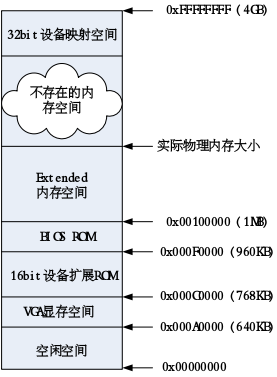
\includegraphics{figures/3.13.1.png}
%\caption{3.13.1.png}
%\end{figure}

图2-1 基于Intel 80386的计算机物理地址空间

处理器处于实模式状态(在86386中,段机制一直存在,可进一步参考2.1.5
【背景】理解保护模式和分段机制),从物理地址0xFFFFFFF0开始执行。初始化状态的CS和EIP确定了处理器的初始执行地址,此时CS中可见部分-选择子(selector)的值为0xF000,而其不可见部分-基地址(base)的值为0xFFFF0000;EIP的值是0xFFF0,这样实际的线性地址(由于没有启动也机制,所以线性地址就是物理地址)为CS.base+EIP=0xFFFFFFF0。在0xFFFFFFF0这里只是存放了一条跳转指令,通过跳转指令跳到BIOS例行程序起始点。更详细的解释可以参考文献{[}1{]}的第九章的9.1节``INITIALIZATION
OVERVIEW''。另外,我们可以通过硬件模拟器qemu来进一步认识上述结果。

\subsubsection{实验2-1:通过qemu了解Intel
80386启动后的CS和EIP值,并分析第一条指令的内容}\label{ux5b9eux9a8c2-1ux901aux8fc7qemuux4e86ux89e3intel-80386ux542fux52a8ux540eux7684csux548ceipux503cux5e76ux5206ux6790ux7b2cux4e00ux6761ux6307ux4ee4ux7684ux5185ux5bb9}

\begin{enumerate}
\def\labelenumi{\arabic{enumi}.}
\item
  启动qemu并让其停到执行第一条指令前,这需要增加一个参数''-S'' qemu --S
\item
  这是qemu会弹出一个没有任何显示内容的图形窗口,显示如下:
\end{enumerate}

%\begin{figure}[htbp]
%\centering
%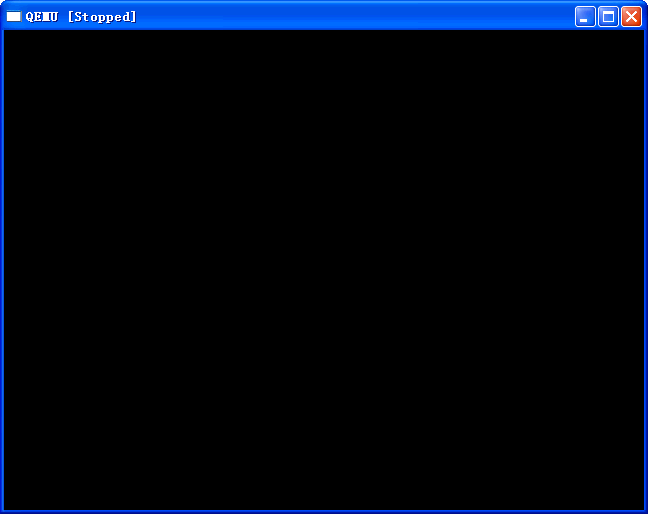
\includegraphics{figures/3.13.2.png}
%\caption{3.13.2.png}
%\end{figure}

\begin{enumerate}
\def\labelenumi{\arabic{enumi}.}
\setcounter{enumi}{2}
\item
  然后通过按''Ctrl+Alt+2''进入qemu的monitor界面,为了了解80386此时的寄存器内容,在monitor界面下输入命令
  ``info registers''
\end{enumerate}

%\begin{figure}[htbp]
%\centering
%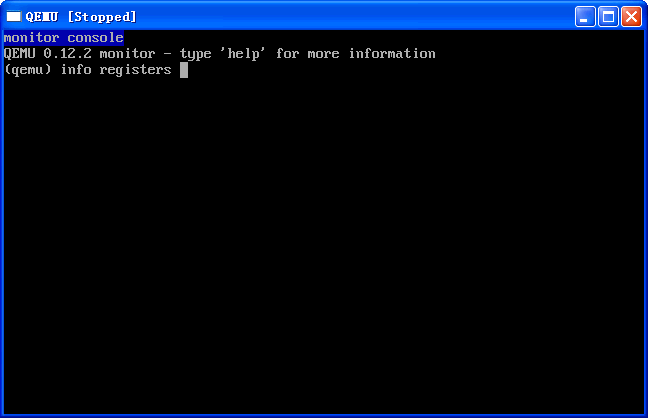
\includegraphics{figures/3.13.3.png}
%\caption{3.13.3.png}
%\end{figure}

\begin{enumerate}
\def\labelenumi{\arabic{enumi}.}
\setcounter{enumi}{3}
\item
  可获得intel 80386启动后执行第一条指令前的寄存器内容,如下图所示
\end{enumerate}

%\begin{figure}[htbp]
%\centering
%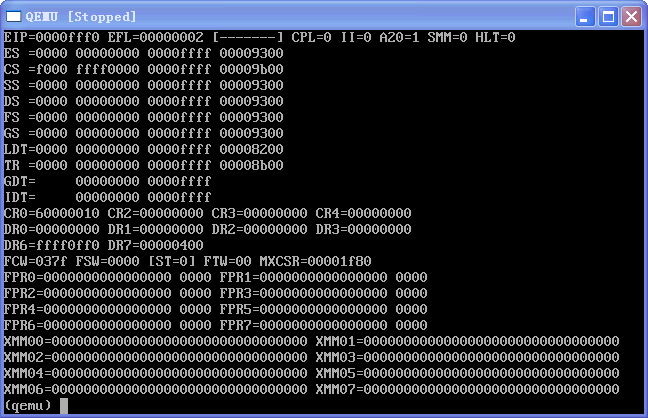
\includegraphics{figures/3.13.4.png}
%\caption{3.13.4.png}
%\end{figure}

从上图中,我们可以看到EIP=0xfff0,CS的selector=0xf000,CS的base=0xfff0000。

BIOS做完计算机硬件自检和初始化后,会选择一个启动设备(例如软盘、硬盘、光盘等),并且读取该设备的第一扇区(即主引导扇区或启动扇区)到内存一个特定的地址0x7c00处,然后CPU控制权会转移到那个地址继续执行。至此BIOS的初始化工作做完了,进一步的工作交给了ucore的bootloader;ucore的bootloader会完成处理器从实模式到保护模式的转换,并从硬盘上读取并加载ucore。其大致流程如下图所示:

%\begin{figure}[htbp]
%\centering
%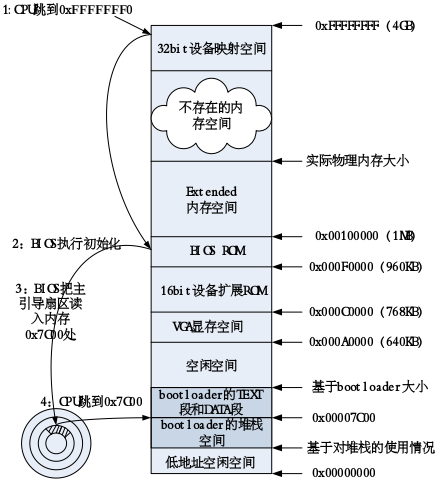
\includegraphics{figures/3.13.5.png}
%\caption{3.13.5.png}
%\end{figure}

图2-2 Intel80386启动过程
